\documentclass[a4paper]{article}
\usepackage{a4wide}
\usepackage[english]{babel}
\usepackage{amsmath,amssymb}
\usepackage{tikz}
\usetikzlibrary{arrows,trees,automata}
\usepackage{aip}%             't beste als aip de laatste in de lijst is.

\usepackage{graphics}
\usepackage{graphicx}
\usepackage{pgf}
%\usepackage{palatino}
\usepackage{amsmath,amssymb}
\usepackage{bm}
\usepackage[english]{babel}
\usepackage{fancybox}
\usepackage{hyperref}

% colors
\def\red#1{{\color{red}#1}}
\def\blue#1{{\color{blue}#1}}
\definecolor{mygreen}{rgb}{0,.5,0}
\def\green#1{{\color{mygreen}#1}}

 % input, general variable
\newcommand{\xvar}{{X}}          % input variable X
\newcommand{\x}{{\mathit{x}}}    % scalar input x
\newcommand{\xv}{{\mathbf{x}}}   % (D x 1) vector input (\x_1, ...,\x_D)^T
\newcommand{\xmat}{{\mathbf{X}}} % (N x D) input matrix 
\newcommand{\xvec}{%             % (N x 1) input vector (N observations) 
	{\ensuremath{\boldsymbol{\mathsf{x}}}}}  
 
% target data
\newcommand{\yvar}{T}          %  target variable 
\newcommand{\y}{{\mathit{t}}}  %  scalar target value 
\newcommand{\yv}{{\mathbf{y}}} %  vector target
\newcommand{\yvec}{%           %  N x 1 target vector
	{\ensuremath{\boldsymbol{\mathsf{t}}}}} 

% latent variables
\newcommand{\zvar}{Z}            % latent variable 
\newcommand{\z}{{\mathit{z}}}    % latent var value 
\newcommand{\zv}{{\mathbf{z}}}   % K x 1 latent variable
\newcommand{\zmat}{{\mathbf{Z}}} % NxK latent var matrix 

% data sets
\newcommand{\data}{\mathcal{D}} % observed data set
\newcommand{\xset}{\{\xv_1,\dotsc,\xv_N\}} % input sequence
\newcommand{\yset}{\{\y_1,\dotsc,\y_N\}}   % target sequence
\newcommand{\xyset}{\{(\xv_1,\y_1),\dotsc,(\xv_N,\y_N)\}} % paired seq

% sequences (ordered sets)
\newcommand{\xseq}[2]{{\xv_{#1},\dotsc,\xv_{#2}}} 
\newcommand{\zseq}[2]{{\zv_{#1},\dotsc,\zv_{#2}}}

% other signals

\newcommand{\class}{{\mathcal{C}}} %  classes
\newcommand{\noise}{{\epsilon}} %  noise	
\newcommand{\noisevec}{%
	{\ensuremath{\boldsymbol{\epsilon}}}} 


%% parameters

\newcommand{\thpar}{{\theta}} % generic parameters
\newcommand{\thvec}{%
	{\ensuremath{\boldsymbol{\theta}}}}
\newcommand{\thold}{{\thvec^{\text{\red{old}}}}}
\newcommand{\thnew}{{\thvec^{\text{\red{new}}}}} 
\newcommand{\thlib}{{\Theta}}

\newcommand{\w}{{\mathit{w}}} % alternative parameter 
\newcommand{\wv}{{\mathbf{w}}} 
\newcommand{\wmat}{{\mathbf{W}}}
\newcommand{\wlib}{{\mathcal{W}}}

% prior
\newcommand{\prio}{{\pi}}
\newcommand{\priovec}{\ensuremath{\boldsymbol{\pi}}}

 % Gaussian pars

\newcommand{\Normal}{\mathcal{N}}
\newcommand{\Bern}{\mathrm{Bern}} % bernouilli

\newcommand{\mupar}{{\ensuremath{\mu}}}
\newcommand{\muvec}{{\ensuremath{\boldsymbol{\mu}}}}

\newcommand{\sgm}{{\sigma}}
\newcommand{\sgmsq}{{\sigma^2}}
\newcommand{\Sgm}{{\ensuremath{\boldsymbol{\Sigma}}}}
\newcommand{\Prec}{{\ensuremath{\boldsymbol{\Lambda}}}}


% prob, expectation, variance
\newcommand{\p}{p} % probability (mass and density)
\newcommand{\Exp}{\mathbb{E}} % expectation
\newcommand{\cov}{\mathrm{cov}} % covariance
\newcommand{\var}{\mathrm{var}} % variance

% chapter 12 on PCA

\newcommand{\vv}{{\mathbf{v}}}   % 
\newcommand{\vmat}{{\mathbf{V}}}   % 
\newcommand{\mv}{{\mathbf{m}}}   % 
\newcommand{\rmat}{{\mathbf{R}}}

% chapter 13 on PCA

\newcommand{\amat}{{\mathbf{A}}}   % 
\newcommand{\cmat}{{\mathbf{C}}} 
\newcommand{\Gambf}{{\ensuremath{\boldsymbol{\Gamma}}}}

% extra math
\newcommand{\realnumbers}{\mathbb{R}}
\newcommand{\beq}{\begin{equation}}
\newcommand{\eeq}{\end{equation}}

\newcommand{\trace}{\mathrm{Tr}}
\newcommand{\diag}{{\mathrm{diag}}}
\newcommand{\zerovec}{{\mathbf{0}}} % 0 vector
\newcommand{\llh}{{\mathit{L}}} % log likelihood
\newcommand{\resp}{\gamma} % responsibility
\newcommand{\Q}{\mathcal{Q}}  % expected complete llh
\newcommand{\KL}{\mathrm{KL}} % Kullback-Leibler divergence
\newcommand{\FreeEnergy}{\mathcal{L}}
\def\d#1{{\,\mathrm{d}#1}} % differential d in integrals
%\newcommand{\d}[1]{{\,\mathrm{d}#1}}





%%%
%%%
%%%

\newcommand{\A}{\mathcal{A}}
\newcommand{\B}{\mathcal{B}}
\newcommand{\C}{\mathcal{C}}
\newcommand{\D}{\mathcal{D}}
\newcommand{\E}{\mathcal{E}}
\newcommand{\I}{\mathcal{I}}
\newcommand{\M}{\mathcal{M}}
\newcommand{\N}{\mathcal{N}}
\newcommand{\X}{\mathcal{X}}
\newcommand{\Y}{\mathcal{Y}}
\newcommand{\mc}[1]{\mathcal{#1}}


% full page graph inclusion 
\newcommand{\incgraph}[1]{\includegraphics[keepaspectratio,width=\textwidth, height=.8\textheight]{#1}}





%colors
%\def\r#1{{\color{red}#1}}
%\def\b#1{{\color{blue}#1}}
%\definecolor{mygreen}{rgb}{0,.5,0}
%\def\g#1{{\color{mygreen}#1}}


\newcommand{\tjboxed}[1]{\par\begin{center}\tikz \node[draw,text width=13cm,inner sep=3pt,line width=1pt] {\parbox{13cm}{#1}};\end{center}}
%\newcommand{\tjboxed}[1]{}

%                        HEADER INFORMATIE
\examendatum{14 April 2011}                    % Datum van het examen.
\examentijd{14h00--17h00}                      % Tijd van het examen.

\begin{document}

\begin{exam}
%
% algemene vorm van invoer:
% gebruik het 'environment'
%       \begin{vraag}{xxx}
%         ...
%       \end{vraag}
% Hierin wordt in xxx beschreven hoe de verschillende onderdelen
% scoren. Per vraag zijn 10 punten te verdelen. Bij het nakijken per
% onderdeel een geheel aantal punten tussen 0 en aangegeven aantal
% toekennen.
%
% Deelvragen worden aangegeven door het environment
% \begin{deelvraag}
%   ...
% \end{deelvraag}
%

% Hier is vraag 1
\begin{vraag}{each sub-question a through e: 2 points. Total 10 points}
For each of the following sub-questions, you are asked to provide
a \emph{short but essential} answer. You should not need more than
three sentences per answer.

\begin{deelvraag}
Consider a binary classification problem with two classes
$\{y_1,y_2\}$ and input vector $x$. We are given a data set to
train the parameters $\theta$ for a likelihood model of the form
$$
p(y_k=1|x,\theta) = \frac{1}{1 + e^{-\theta_k^T x}}
$$
There a two fundamentally different ways to train $\theta$, namely through a generative model or by discriminative training.\\
(1) Explain shortly how we train $\theta$ through a generative model. No need to work out all equations for Gaussian models, but explain the strategy in probabilistic modeling terms.\\
(2) Explain shortly how we train $\theta$ through a discriminative
approach. % What are the consequences for $\theta$ relative to the generative approach?
 \tjboxed{
(1) In a generative model, the class posterior is obtained through
Bayes rule,
$$
p(y_k=1|x,\theta) \propto p(x|y_k=1,\theta) p(y_k=1|\theta)
$$
In terms of ML training, this means we maximize the \emph{joint} log-likelihood $\sum_n \log p(x_n,y_n|\theta)$ wrt $\theta$. This leads to a structured breakdown of the model (and parameters) into a class-conditional likelihood $ p(x|y_k=1,\theta) $ and class priors $p(y_k=1|\theta)$. \\
(2) In a discriminative model, the posterior class density
$ p(y_k=1|x,\theta) $  is directly trained, i.o.w. we maximize the
\emph{conditional} log-likelihood $\sum_n \log p(y_{nk}|x_n\theta)$.
There's no structured model breakdown.
} % end tjboxed
\end{deelvraag}

\begin{deelvraag}
    Explain shortly how Bayes rule relates to machine learning. In your answer, you may assume a model $\mathcal{M}$ with prior distribution $p(\mathcal{M})$ and an observed data set $D$.
\tjboxed{ 
$$ \underbrace{p(\mathcal{M}|D)}_{\text{posterior}} = \frac{p(D|\mathcal{M})}{p(D)}\underbrace{p(\mathcal{M})}_{\text{prior}}
$$
Bayes rule relates what we know about a model before (prior) and
after (posterior) having seen the data. The difference between the
prior and posterior distributions for the model can be interpreted
as a `machine learning' effect. (Alternative answers are also
possible).
} % end tjboxed
\end{deelvraag}

\begin{deelvraag}
What is the difference between supervised and unsupervised learning? Express the goals of these two learning methods in terms of a probability distribution. (I'm looking here for a statement such as: " Given $\ldots$, the goals of supervised/unsupervised learning is to estimate $p(\cdot|\cdot)$".)

 \tjboxed{
Given data $D=\{(x_1,y_1),\ldots,(x_N,y_N)\}$ and a model $p(y|x,\theta)$, the goal of supervised learning is to estimate $p(\theta|D)$. Given data $D=\{x_1,\ldots,x_N\}$ and a model $p(x|\theta)$, the goal of unsupervised learning is to estimate $p(\theta|D)$. 
} % end tjboxed
\end{deelvraag}




\begin{deelvraag}

In a particular model with hidden variables, the log-likelihood
can be worked out to the following expression:
$$
 L(\theta;D) = \sum_n \log \left(\sum_k
\pi_k\,\N(x_n|\mu_k,\Sigma_k)\right)
$$
Do you prefer a gradient descent or EM algorithm to estimate maximum likelihood values for the parameters?  Explain your answer. (No need to work out the equations. )

\tjboxed{ Since this
expression does not degenerate into simple MVGs, the EM approach
is in practice preferred.
} % end tjboxed
\end{deelvraag}

\begin{deelvraag}
The maximum likelihood estimate (MLE) of the class-conditional
mean in a classification problem can be expressed as
$$
\hat\mu_k = \frac{\sum_n y_n^k x_n}{\sum_n y_n^k}
$$
and the M-step update for the cluster mean in a clustering problem
is given by
$$
\hat\mu_k = \frac{\sum_n \resp_n^k x_n}{\sum_n \resp_n^k}
$$
Explain the relation between $y_n^k$ and $\resp_n^k$. Is $y_n^k$ a
binary variable? And what about $\resp_n^k$?

\tjboxed{ 
$y_n^k$ are \emph{binary} indicator variables, given by
$$
y_n^k = \begin{cases} 1 & \text{if}\quad Y_n=k \\ 0 & \text{else
}\end{cases}
$$
$\resp_n^k$ are \emph{soft} indicators, given by $\resp_n^k =
p(Z_n=k|x_n,\theta)$, where $Z_n$ refers to the unobserved $n$th
class label.
} % end tjboxed

\end{deelvraag}

\end{vraag}

% Hier is vraag 2

\begin{vraag}{a) 2 points; b) 1 point; c) 2 points; d) 2 points; e) 1 point; f) 1 point; g) 1 point. Total 10 points}

The lifetime $x>0$ of a light bulb is postulated to be exponentially distributed with unknown mean
$\mu>0$, i.e.
$$
p(x|\mu) = \frac{1}{\mu} \,e^{-x/\mu}
$$
In order to estimate $\mu$, the lifetimes $\mathbf{X}=\{x_1,\ldots,x_N\}$ of $N$ independent bulbs are observed.

\begin{deelvraag}
Work out the log-likelihood $\log p(\mathbf{X}|\mu)$.

\tjboxed{
\begin{eqnarray}
\log \, \prod_{n=1}^N p(x_n|\mu) &=& \sum_n \log \left(\frac{1}{\mu}\, \exp(-\frac{x_n}{\mu})\right) \nonumber \\
&=& -N\log \mu -\frac{1}{\mu}\sum_n x_n \nonumber \\
&=& -N \left( \log \mu + \frac{\bar{x}}{\mu}\right) \nonumber
\end{eqnarray}
}% end tjboxed

\end{deelvraag}

\begin{deelvraag}
What is the maximum likelihood estimate for $\mu$ based on observations $\mathbf{X}$?

\tjboxed{$\mu = \bar{x}$}
\end{deelvraag}

In a separate experiment M independent bulbs were tested, but the
individual lifetimes were not recorded. We will use the symbols
$\mathbf{Z} = \{z_{1},\dots,z_{M}\}$ for the \emph{unobserved} lifetimes of bulbs
$N+1,\ldots,N+M$ and $\{\mathbf{X},\mathbf{Z}\} =\{x_1,\ldots,x_N,z_1,\ldots,z_M\}$ for
the complete data set. Instead of lifetimes, we only recorded if a
bulb had failed at time $t$. We record $y_m=1$ if bulb $N+m$ still
burned at time $t$ and $y_m=0$ if the bulb had already failed at
time $t$. We will now derive an EM algorithm to estimate $\mu$,
based all $N+M$ observations.


\begin{deelvraag}
Complete the following two formula's for the EM algorithm:
\begin{align*}
\textbf{E-step}&:\; &&\text{evaluate } p(\cdot|\cdot,\mu^{\mathrm{old}}) \\
\textbf{M-step}&:\; &&\mu^{\mathrm{new}} = \arg\max_{\cdot} \sum_{\cdot} p(\cdot|\cdot,\cdot) \log p(\cdot,\cdot|\cdot)
\end{align*} 
 \tjboxed{
\textbf{E-step}: evaluate $p(\mathbf{Z}|\mathbf{X},\mu^{\mathrm{old}})$\\
 \textbf{M-step}: $\mu^{\mathrm{new}} = \arg\max_{\mu} \sum_{\mathbf{Z}} p(\mathbf{Z}|\mathbf{X},\mu^{\mathrm{old}}) \log p(\mathbf{Z},\mathbf{X}|\mu)$
}
\end{deelvraag}

\begin{deelvraag}
Proof that the expected complete-data log-likelihood $\mathbb{E}[\log p(\mathbf{X},\mathbf{Z}|\mu)]$ equals
$$
-(N+M)\log \mu -\frac{1}{\mu}\left(N\bar{x} + \sum_{m=1}^M \mathbb{E}[z_m]\right)
$$
where $\bar{x} = \frac{1}{N}\sum_{n=1}^N x_n$. 
\tjboxed{\begin{eqnarray}
\log p(\mathbf{X},\mathbf{Z}|\mu) &=& \log \left( \prod_{n=1}^N p(x_n|\mu) \, \prod_{m=1}^M p(z_m|\mu) \right)  \nonumber \\
&=& \sum_{n=1}^N  \, \log \left(\frac{1}{\mu}\, \exp(-\frac{x_n}{\mu})\right) + \sum_{m=1}^M \, \log \left(\frac{1}{\mu}\, \exp(-\frac{x_n}{\mu})\right) \nonumber \\
&=& -(N+M)\log \mu -\frac{1}{\mu}\left(N\bar{x} + \sum_{m=1}^M z_m\right) \nonumber \\
\mathbb{E}[p(\mathbf{X},\mathbf{Z}|\mu)] &=&  -(N+M)\log \mu -\frac{1}{\mu}\left(N\bar{x} + \sum_{m=1}^M \mathbb{E}[z_m]\right) \nonumber
\end{eqnarray}
}% end tjboxed
\end{deelvraag}

\begin{deelvraag}
You can find the (local) optimum of $\mathbb{E}[\log p(\mathbf{X},\mathbf{Z}|\mu)]$ by setting its derivative w.r.t. $\mu$ to zero. Now differentiate $\mathbb{E}[\log p(\mathbf{X},\mathbf{Z}|\mu)]$ (see answer 2d) w.r.t. $\mu$ and set to zero to obtain the re-estimation formula (\textbf{M-step}) for $\mu$.
\tjboxed{
$$
{\partial \over \partial \mu} \mathbb{E}[p(\mathbf{X},\mathbf{Z}|\mu)] = -\frac{N+M}{\mu} + \frac{1}{\mu^2}\left(N\bar{x} + \sum_{m=1}^M \mathbb{E}[z_m] \right) 
$$
Set to zero to obtain
$$
\mu = \frac{1}{N+M}\left(N\bar{x} + \sum_{m=1}^M \mathbb{E}[z_m] \right)
$$
}% end tjboxed
\end{deelvraag}


\medskip
We do not derive the $\mathbb{E}[z_m]$ for the \textbf{E-step}. Use the following equation instead
\begin{eqnarray}
\mathbb{E} [z_m] = \left\{
\begin{array}{ll}
t+\mu & \text{if }y_m=1 \\
\mu - \frac{t\exp\left(-\frac{t}{\mu}\right)}{1-\exp\left(-\frac{t}{\mu}\right)} & \text{if }y_m=0 \\
\end{array} \right. \nonumber
\end{eqnarray}
\begin{deelvraag}
In total we found that $r$ out of $M$ bulbs had failed at time $t$. Derive an expression for $\sum_{m=1}^M \mathbb{E}[z_m]$ in terms of $r$ and $M$.  
\tjboxed{
$$
\sum_{m=1}^M \mathbb{E}[z_m] = (M-r)(t+\mu^{\mathrm{old}})+r\left(\mu^{\mathrm{old}} - \frac{t\exp\left(-\frac{t}{\mu^{\mathrm{old}}}\right)}{1-\exp\left(-\frac{t}{\mu^{\mathrm{old}}}\right)}\right)
$$
}% end tjboxed
\end{deelvraag}

\begin{deelvraag}
Put the results of the last two exercises together and derive the re-estimation formula (\textbf{M-step}) for $\mu$ (in terms of a previous estimate of $\mu^{\mathrm{old}}$).
\tjboxed{
$$
\mu^{\mathrm{new}} = \frac{1}{N+M}\left(N\bar{x} + (M-r)(t+\mu^{\mathrm{old}})+r\left(\mu^{\mathrm{old}} - \frac{t\exp\left(-\frac{t}{\mu^{\mathrm{old}}}\right)}{1-\exp\left(-\frac{t}{\mu^{\mathrm{old}}}\right)}\right) \right)
$$
}
\end{deelvraag}

\end{vraag}


%%%%%%%%%%%%%%%%
%%%
%%% MDL vragen
%%%

%%%
%%% Vraag Laplace
%%%
\begin{vraag}{a) 1 point; b) 5 points. Total 6 points}
    Let $B$ be a positive real valued random variable with probability
    density
    \[ p_B(b) = e^{-b},\quad\text{for all $b>0$}. \]
    Also $A$ is a real valued random variable with conditional
    density
    \[ p_{A|B}(a|b) = \sqrt{\frac{b}{\pi}}e^{-a^2b},\quad\text{for
    all $a\in(-\infty,\infty)$ and $b\in(0,\infty)$}. \]
    \begin{deelvraag}
        Give an (integral) expression for $p_A(a)$.\\
        Do not try to evaluate the integral.
        \tjboxed{
            \[ p_A(a) = \int_0^{\infty} p_B(b)p_{A|B}(a|b)\,db =
                \int_0^{\infty}
                \sqrt{\frac{b}{\pi}}e^{-b(a^2+1)}\,db \]
        }
    \end{deelvraag}
    \begin{deelvraag}
        Approximate $p_A(a)$ using the Laplace approximation.\\
        Give the detailed derivation, not just the answer.
        \tjboxed{
            First we define for notational efficiency
            \[ f_a(b) = \sqrt{\frac{b}{\pi}}e^{-b(a^2+1)}. \]
            In order to find the maximum we take the first
            derivative w.r.t.\ $b$.
            \begin{align*}
                \frac{\partial}{\partial b}f_a &=
                \frac{1}{2\pi}\sqrt{\frac{\pi}{b}}e^{-b(a^2+1)}-\sqrt{\frac{b}{\pi}}(a^2+1)e^{-b(a^2+1)}
                \\
                &= e^{-b(a^2+1)}\left( \frac12\sqrt{\frac{1}{\pi b}}-(a^2+1)\sqrt{\frac{b}{\pi}}
                \right) \\
            \intertext{Solving for zero we get}
                \frac12\sqrt{\frac{1}{\pi b}} &=
                (a^2+1)\sqrt{\frac{b}{\pi}} \\
                \sqrt{\frac{1}{b^2}} &= \frac{1}{b} = 2(a^2+1) \\
                b_{\text{opt}} &= \frac{1}{2(a^2+1)}
            \end{align*}
        }%tjboxed
        \tjboxed{
            For the Laplace approximation we need the (negative of
            the) second derivative w.r.t.\ $b$ of $\ln f_a(b)$,
            evaluated in $b_{\text{opt}}$.
            \begin{align*}
                g_a(b) &= \ln f_a(b) = -b(a^2+1) +
                    \frac12\ln\frac{b}{\pi}. \\
                \frac{\partial}{\partial b} g_a(b) &= -(a^2+1) +
                    \frac12\frac{\pi}{b}\frac{1}{\pi} = -a^2-1 +
                    \frac{1}{2b} \\
                \frac{\partial^2}{\partial b^2} g_a(b) &= -\frac{1}{2b^2}
                    \\
                A_{\text{Laplace}} &= \frac{1}{2b_{\text{opt}}^2} =
                    2(a^2+1)^2.
            \end{align*}
        }%tjboxed
        \tjboxed{
            So we find
            \begin{align*}
                p_A(a)  &= \int_0^{\infty} f_a(b)\,db \\
                        &\approx
                            f_a(b_{\text{opt}})\sqrt{\frac{2\pi}{A_{\text{Laplace}}}}
                            \\
                        &= \sqrt{\frac{1}{2e}}\frac{1}{(a^2+1)^{\frac32}}
                        \\
                        &= 1.16582\frac{1}{(a^2+1)^{\frac32}}
                            \\
                \intertext{Compare this to the actual value !}
                p_A(a) &= \int_0^{\infty} f_a(b)\,db \\
                        &= \frac{1}{2}\frac{1}{(a^2+1)^{\frac32}}
            \end{align*}
        }%tjboxed
    \end{deelvraag}
\end{vraag}



%%%
%%% Vraag BIC,MDL begrip
%%%
\newcommand{\tjM}{\ensuremath{\mathcal{M}}}
\newcommand{\tjpar}{\ensuremath{\theta}}
\newcommand{\tjparv}{\ensuremath{\underline{\theta}}}
\newcommand{\tjdat}{\ensuremath{d}}
\newcommand{\tjdatx}{\ensuremath{x^N}}
\begin{vraag}{a) 4 points; b) 2 points; c) 2 points. Total 8 points} % 5
The \emph{Bayesian Information Criterion} is results in
\[
 \underbrace{\log\frac{p(\tjM_1|\tjdatx)}{p(\tjM_2|\tjdatx)}}_{(*1)} \approx 
  \underbrace{\log\frac{p(\tjM_1)}{p(\tjM_2)}}_{(*2)} +
  \underbrace{\log\frac{p(\tjdatx|\tjM_1,\hat{\tjparv}_1)}{p(\tjdatx|\tjM_2,\hat{\tjparv}_2)}}_{(*3)} +
  \underbrace{\frac12\left(k_1-k_2\right)\log N}_{(*4)}.
\]
Here \tjdatx{} is a binary data sequence of length $N$, $k_1$ and $k_2$ are the number of free parameters in respectively model $\tjM_1$ and $\tjM_2$, and $\hat{\tjparv}_1$ and $\hat{\tjparv}_2$ are the estimated (ML) parameter vectors.
\begin{deelvraag}
  Explain the four terms marked by (*1), (*2), (*3), and (*4).
  \tjboxed{(*1) This ratio of model posteriors (given the data) allows us to select the most appropriate model of the two options.}
  \tjboxed{(*2) This ratio shows our initial preference of the first model relative to the second one.}
  \tjboxed{(*3) This is the log-likelihood ratio of the two models after observing the data.}
  \tjboxed{(*4) This is the correction term needed to compare models of different complexity.}
\end{deelvraag}
\begin{deelvraag}
The binary data $\tjdatx=x_1,x_2,\ldots,x_N$ is generated by a Bernoulli process, i.e.
\[p(\tjdatx|\tjM,\tjpar) = (1-\tjpar)^{n(0|\tjdatx)}\tjpar^{n(1|\tjdatx)}. \]
The parameter prior $p(\tjpar|\tjM)$ is given by the Beta distribution:
\[p(\tjpar|\tjM) = \frac{1}{\pi}\frac{1}{\sqrt{\tjpar(1-\tjpar)}}. \]
Let $N=10$ and $x^{10}=1001101101$. Determine $p(\tjdatx|\tjM)$. Give the complete derivation starting with the information given above.
\tjboxed{
  \begin{align*}
    p(\tjdatx|\tjM) &= \int_0^1 p(\tjpar|\tjM) p(\tjdatx|\tjM,\tjpar)\,d\tjpar, \\
      &= \int_0^1 \frac{1}{\pi}\frac{1}{\sqrt{\tjpar(1-\tjpar)}} (1-\tjpar)^4\tjpar^6 \,d\tjpar, \\
      &= \frac{\Gamma(4+\frac12)\Gamma(6+\frac12)}{\pi\Gamma(11)}, \\
      &= \frac{\frac12\frac32\frac52\frac72\cdot\frac12\frac32\frac52\frac72\frac92\frac{11}{2}}{10!}, \\
      &= \frac{77}{262144} = 0.0002937.
  \end{align*}
}
\end{deelvraag}
\begin{deelvraag}
  Why do we think that the probability estimate $p(\tjdatx|\tjM)$ is a useful and good estimate for the actual,
  but unknown, probability $p(\tjdatx|\tjM,\tjpar)$? And how close will $p(\tjdatx|\tjM)$ be to the probability
  $p(\tjdatx|\tjM,\tjpar)$, for any \tjdatx{} and any \tjpar{}, if \tjM{} is a binary memoryless model?
  \tjboxed{
    In the lecture noted it is shown that for the memoryless binary model, with any parameter value \tjpar{}
    and any sequence \tjdatx{} holds
    \[ \log\frac{p(\tjdatx|\tjM,\tjpar)}{p(\tjdatx|\tjM)} \leq \frac12 \log N + 1. \]
    And with the \emph{Capacity-Redundancy theorem} we know that
    \[ \log\frac{p(\tjdatx|\tjM,\tjpar)}{p(\tjdatx|\tjM)} \geq \frac12 \log N - \epsilon_N. \]    
    Here $\epsilon_N\rightarrow0$ as $N\rightarrow\infty$.\\
    So, in this sense, the probability estimate is optimal.
  }
\end{deelvraag}
\end{vraag}

%%% Vraag MDL
%%%

\begin{vraag}{a) 1 point; b) 2 points; c) 3 points. Total 6 points}
	Consider the following binary finite state model (Markov source). This model produces outputs $X_t$ where
	the probability of the next output symbol depends on the current state of the source. We list all non-zero probabilities.
	\begin{align*}
		\Pr\{X_t=0,S_{t+1}=B|S_t=A\} &= 1, \\
		\Pr\{X_t=0,S_{t+1}=A|S_t=B\} &= 0.5, \\
		\Pr\{X_t=1,S_{t+1}=B|S_t=B\} &= 0.5, 
	\end{align*}
	The following figure depicts this model.
	\begin{center}
		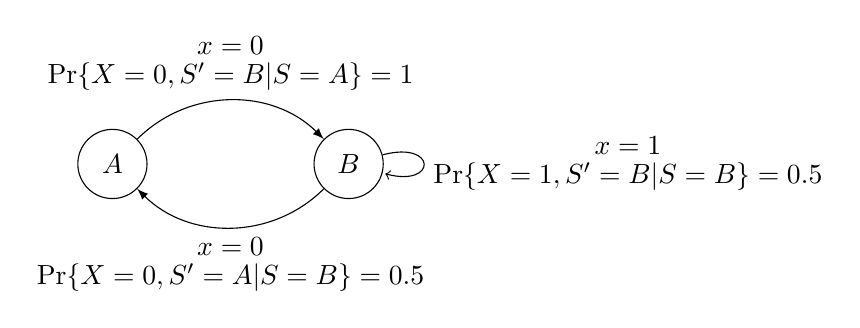
\begin{tikzpicture}[node distance=3cm,bend angle=45]
			\node[state] (A) {$A$};
			\node[state] (B) [right of=A] {$B$};
			\path[-latex] 	(A) edge[bend left] node[above] {\shortstack{$x=0$\\$\Pr\{X=0,S'=B|S=A\}=1$}} (B)
							(B) edge[bend left] node[below] {\shortstack{$x=0$\\$\Pr\{X=0,S'=A|S=B\}=0.5$}} (A)
								edge[loop right] node[right] {\shortstack{$x=1$\\$\Pr\{X=1,S'=B|S=B\}=0.5$}} ();
		\end{tikzpicture}
	\end{center}
	\begin{deelvraag}
		Compute the stationary probabilities $q(A)$ and $q(B)$ where
		\[ q(s) = \lim_{t\rightarrow\infty} \Pr\{S_t=s\}\qquad\text{for }s\in\{A,B\}. \]
%		Note that $q(s)$ can be determined from the equations
%		\[ q(s) = \sum_{s'\in\{A,B\}} q(s')\Pr\{S_{t+1}=s|S_t=s'\}, \]
%		and $q(A)+q(B)=1$.
	\end{deelvraag}
	\tjboxed{%
		\begin{align*}
			q(A) &= \frac{1}{2}q(B), \\
			q(B) &= 1-q(A)
		\end{align*}
		This results in $q(A)=\frac13$ and $q(B)=\frac23$.
	}
	\begin{deelvraag}
		Compute the following probabilities assuming that the model is stationary (i.e.\ $\Pr\{S_1=A\}=q(A)$ and $\Pr\{S_1=B\}=q(B)$).
%		In this case we have for every binary sequence $x^i$
%		\[ \Pr\{X^i=x^i\} = \sum_{s\in\{A,B\}} q(s) \Pr\{X^i=x^i|S_1=s\}. \]
%		Now compute
		\begin{align*}
			&\Pr\{X_1=1\} \\
			&\Pr\{X_2=1|X_1=0\}
		\end{align*}
	\end{deelvraag}
	\tjboxed{%
		\begin{align*}
			\Pr\{X_1=1\} &= q(A)\cdot0 + q(B)\cdot\frac12 = \frac13. \\
		\intertext{For the next one we need}
			\Pr\{X^2=01\} &= q(A)\cdot1\cdot\frac12 + q(B)\cdot\frac12\cdot0 = \frac16, \\
		\intertext{and we find}
			\Pr\{X_2=1|X_1=0\} &= \frac{\Pr\{X^2=01\}}{\Pr\{X_1=0\}} = \frac{1/6}{2/3}=\frac14.
		\end{align*}
	}
	\newcommand{\Ma}{{\mathcal M}_0}
	\newcommand{\tha}{\underline{\theta}_0}
	\newcommand{\Mb}{{\mathcal M}_1}
	\newcommand{\thb}{\underline{\theta}_1}
	\newcommand{\Mc}{{\mathcal M}_2}
	\newcommand{\thc}{\underline{\theta}_2}
	\newcommand{\Mi}{{\mathcal M}_i}
	\newcommand{\thi}{\underline{\theta}_i}
	\begin{deelvraag}
		Let $\Ma$ be the i.i.d.{} model with
		\[ \tha = \left( \Pr\{X_1=1\}\right). \]
		Also $\Mb$ is the first order model with
		\[ \thb = (\theta_{10},\theta_{11}) = \left( \Pr\{X_2=1|X_1=0\},\Pr\{X_2=1|X_1=1\} \right). \]
		And $\Mc$ is the second order model with
		\begin{align*}
			\thc &= (\theta_{200},\theta_{201},\theta_{210},\theta_{211}) \\
			&=\left( \Pr\{X_3=1|X_1=0,X_2=0\},\Pr\{X_3=1|X_1=0,X_2=1\}, \right. \\
			&\qquad\qquad \left.\Pr\{X_3=1|X_1=1,X_2=0\},\Pr\{X_3=1|X_1=1,X_2=1\} \right).
		\end{align*}
		The Markov model produces a `typical' sequence so
		\[ -\log_2\Pr\{X^n=x^n|\Mi,\thi\} \approx H_i(X^n), \]
		where $H_i(X^n)$ is the entropy rate of the $i^{\text{th}}$ model.\\
		Given is that
		\begin{align*}
			H_0(X^n) &= 0.9183\cdot n\\
			H_1(X^n) &= 0.8742\cdot n\\
			H_2(X^n) &= 0.7925\cdot n
		\end{align*}
		\textbf{Determine for what range  of $n$ you should use $\Ma$.} And when $\Mb$ and when $\Mc$?\\
		Use the idea of stochastic complexity and \textbf{motivate your answer}.
	\end{deelvraag}
	\tjboxed{%
		The remaining conditional probabilities should be computed in order to find the entropies.
		\\[\baselineskip]
		Then we find the stochastic complexities
		\begin{align*}
			S.C._0 &= \frac{\log_2n}{2} + 0.9183\cdot n \\
			S.C._1 &= \frac{2\log_2n}{2} + 0.8742\cdot n \\
			S.C._2 &= \frac{4\log_2n}{2} + 0.7925\cdot n
		\end{align*}
		Equality of $S.C._0$ and $S.C._1$ happens at $n=69\sim70$.\\
		Equality of $S.C._1$ and $S.C._2$ happens at $n=76\sim77$.
		\\[\baselineskip]
		So up to $n=70$ we use $\Ma$, then until $n=77$ we use $\Mb$ and afterwards we use $\Mc$.
	}
\end{vraag}

%\newpage
%\section*{Appendix: formula sheet}
%
%Consider random variables (RV) $x\in\mathcal{X}$ and $y\in \mathcal{Y}$. The basic axioms of probability theory are the sum and product rules,
%$$
%p(x) + p(\overline{x}) = 1 \quad \text{(sum rule)}
%$$
%$$
%p(x,y) = p(x|y)p(y) \quad \text{(product rule)}
%$$
%
%The following formulas can be derived from the sum and product rules,
%$$
%p(x|y) = \frac{p(x,y)}{p(y)} \quad \text{(conditional probability of $x$, given $y$)}
%$$
%
%$$
%p(x|y) = \frac{p(y|x)p(x)}{p(y)} = \frac{p(y|x)p(x)}{\sum_{x\in\mathcal{X}}p(y|x)p(x)} \quad \text{(Bayes rule)}
%$$
%
%$$
%p(x) = \sum_{y\in\mathcal{Y}} p(x,y) \quad \text{(marginal probability)}
%$$
%
%\medskip
%We use for mean and variance the following notation,
%
%$$
%\varepsilon[x] = \langle x \rangle = \int_x x p(x) \d{x} \quad \text{(expectation)}
%$$
%$$
%\var[x] = \varepsilon[(x-\varepsilon[x])(x-\varepsilon[x])^T] \quad \text{(variance)}
%$$
%\medskip
%\textbf{Some probability distributions}\\
%The \emph{Bernoulli distribution} is a discrete distribution having two possible outcomes labeled by $x = 0$
%and $x = 1$ in which $x = 1$ ("success") occurs with probability $\theta$ and $x = 0$ ("failure") occurs
%with probability $1-\theta$. It therefore has probability function
%\begin{equation}
%p(x|\theta) =\theta^x(1-\theta)^{1-x}
%\tag{A.1}
%\end{equation}
%
%The \emph{Gaussian distribution} with mean $\mu$ and variance $\sigma^2$ is defined as
%$$
%\N(x|\mu,\sigma^2) = \frac{1}{\sqrt{2\pi}\sigma} \exp\left\{-\frac{1}{2\sigma^2}(x-\mu)^2\right\}
%$$
\end{exam}
\end{document}
